\section{ggplot2 - Part 3}
\subsection{statistics in ggplot2}
\begin{frame}\frametitle{Statistics}
  \begin{itemize}
  \item useful to transform your data before plotting, and that's what statistical transformations do
  \item name convention \texttt{stat\_specification}
  \item every statistic has a default geometry, e.g. \texttt{stat\_bin()} uses \texttt{geom\_bar()}
  \end{itemize}
\end{frame}


\begin{frame}[allowframebreaks,fragile]\frametitle{\texttt{stat\_bin()}}
  \begin{itemize}
  \item bins (and counts) (grouped) data 
  \end{itemize}
\small
\begin{verbatim}
> ggplot(data,aes(x=EC1)) +
+     geom_bar() +
+     stat_bin(geom="text", aes(label=..count..),
+              colour="red", size=14, vjust=1)
ymax not defined: adjusting position using y instead
\end{verbatim}
\begin{center}
  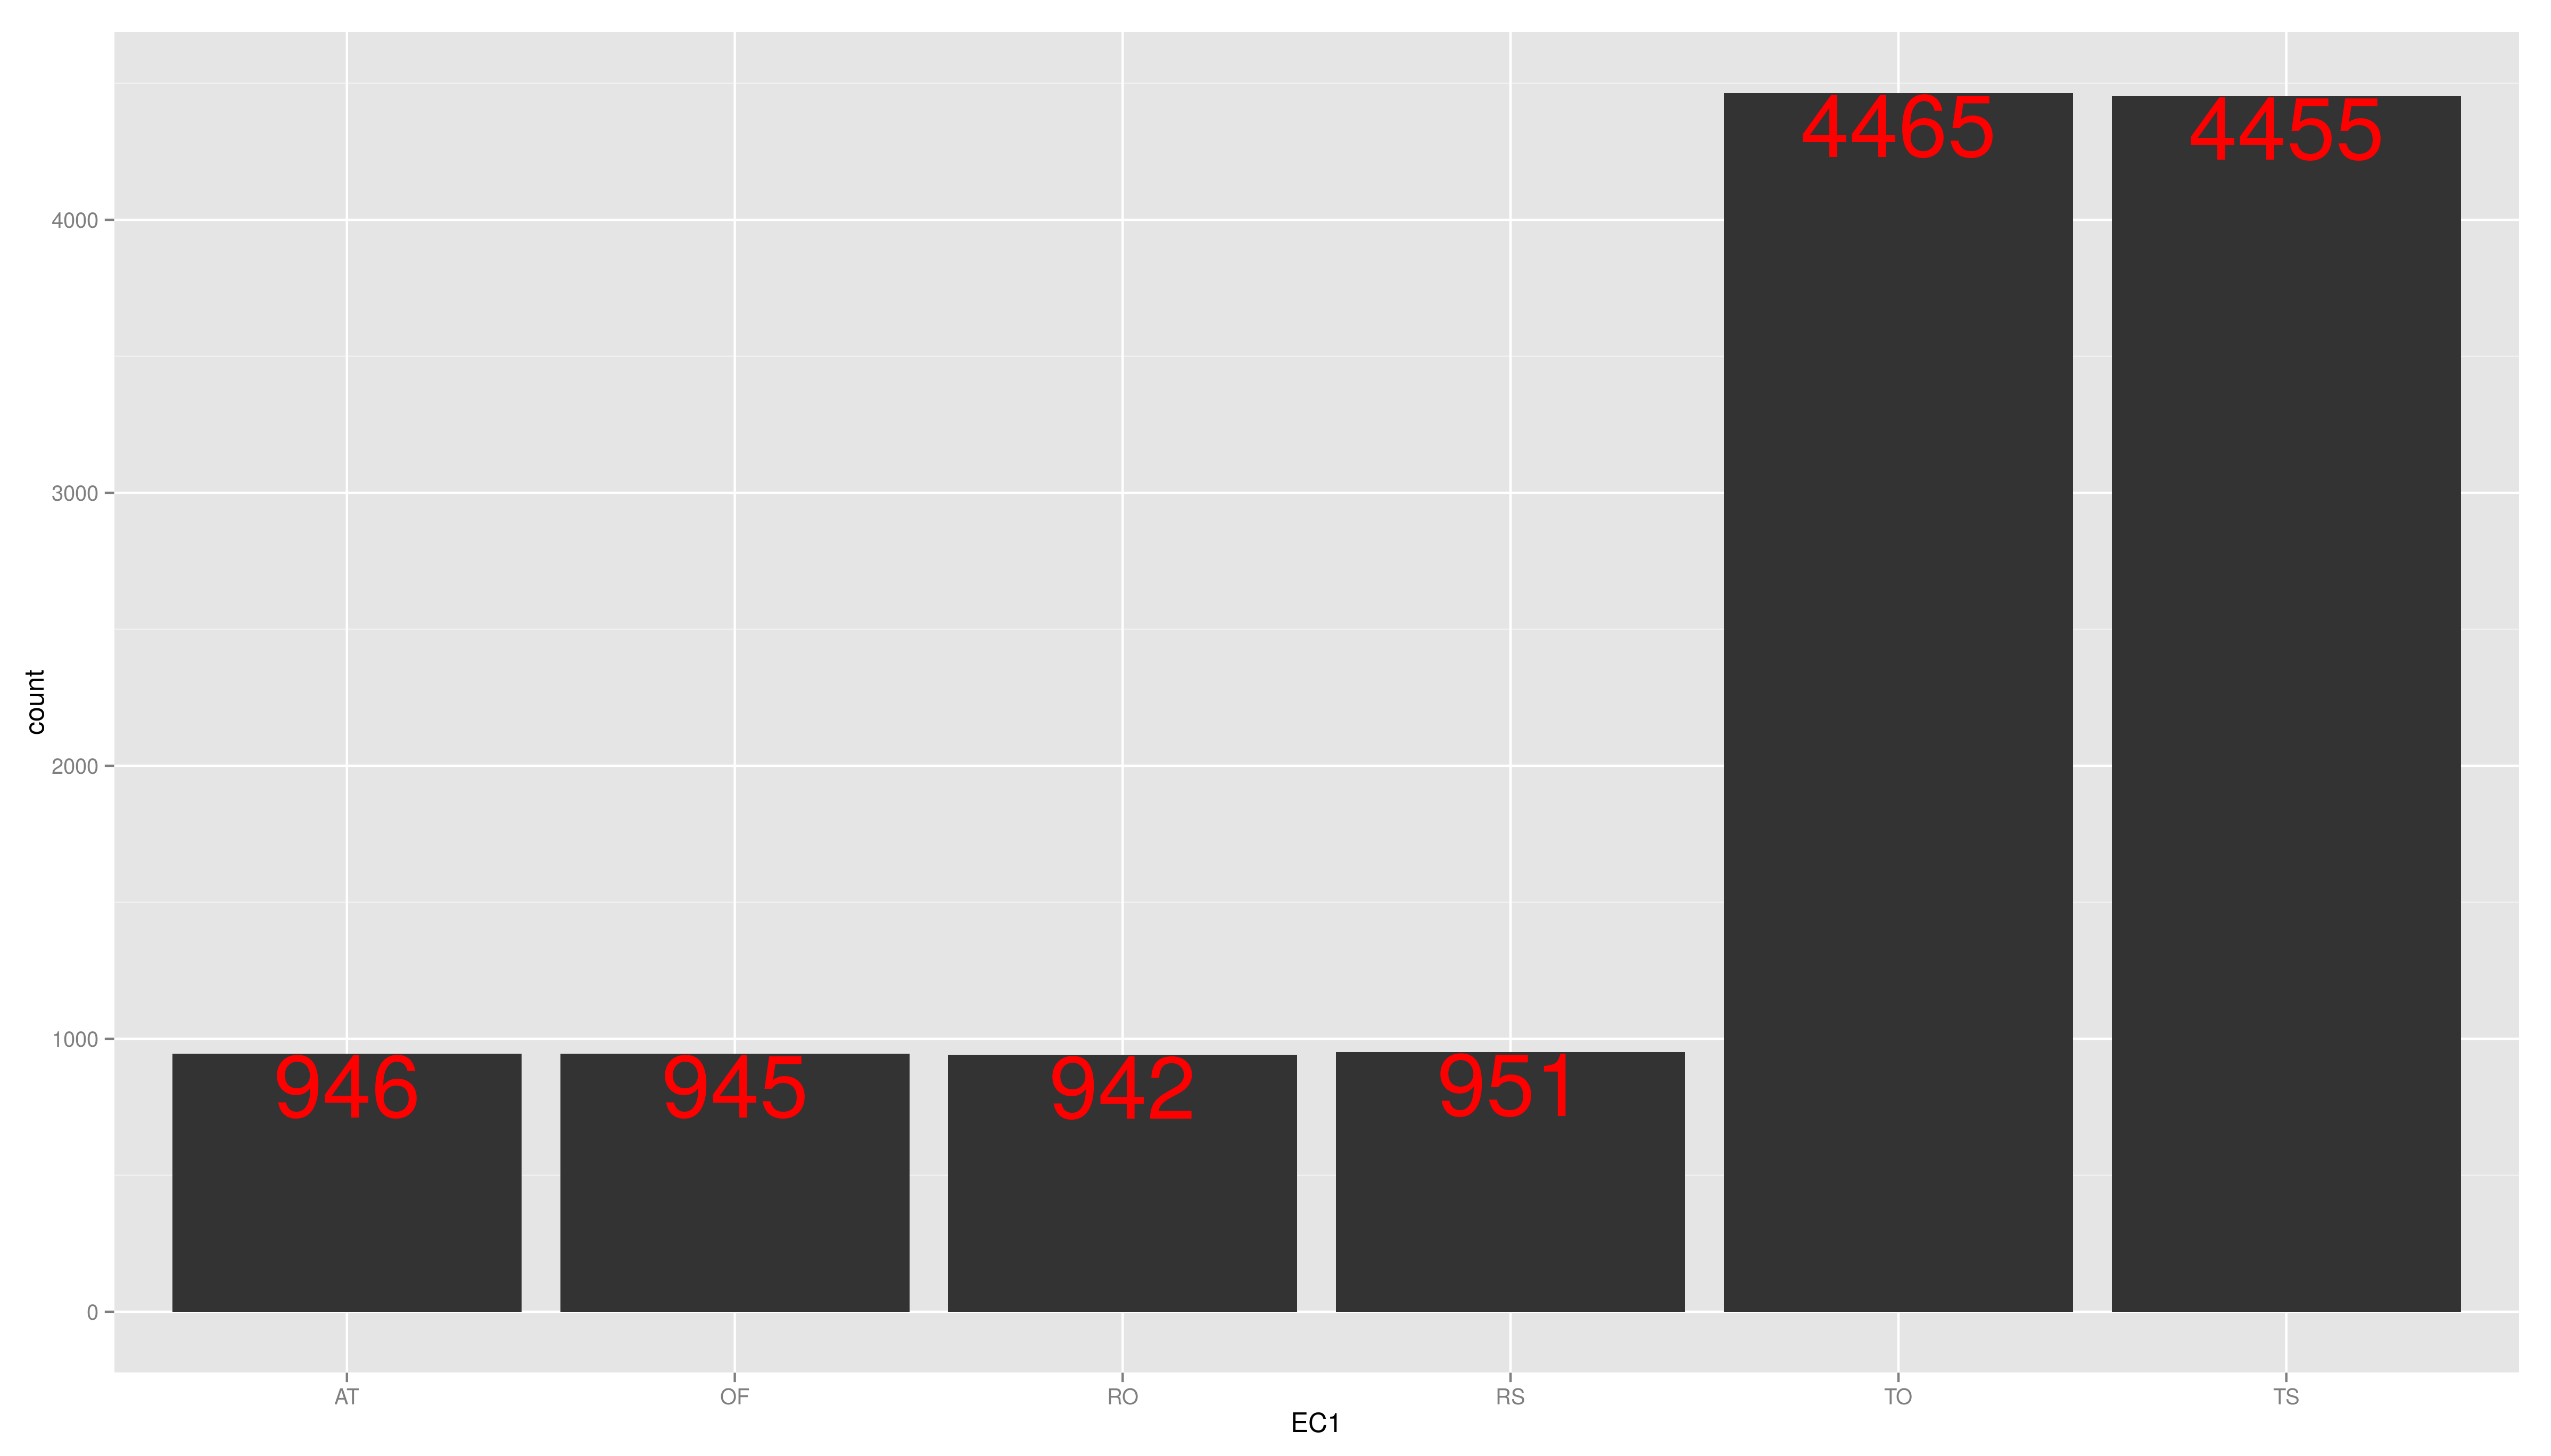
\includegraphics[width=6.5cm]{statbin.png}
\end{center}
\end{frame}


\begin{frame}[allowframebreaks,fragile]\frametitle{\texttt{stat\_density()} \& \_function()}
\texttt{stat\_density()}
  \begin{itemize}
  \item computes and plots density estimates
  \item allows different kernels and bandwidths
  \item default geometry: \texttt{geom\_density()}
  \end{itemize}
\texttt{stat\_function()}
  \begin{itemize}
  \item plots functions, needs only one aesthetic: \texttt{y}
  \item default geometry: \texttt{geom\_path()}
  \end{itemize}
\small
\begin{verbatim}
> ggplot(data,aes(x=log(TTime))) +
+     geom_density() +
+     stat_function(fun=dnorm,
+                   args = list(mean=mean(log(data$TTime)),
+                               sd=sd(log(data$TTime)))
+                   )
\end{verbatim}
\begin{center}
  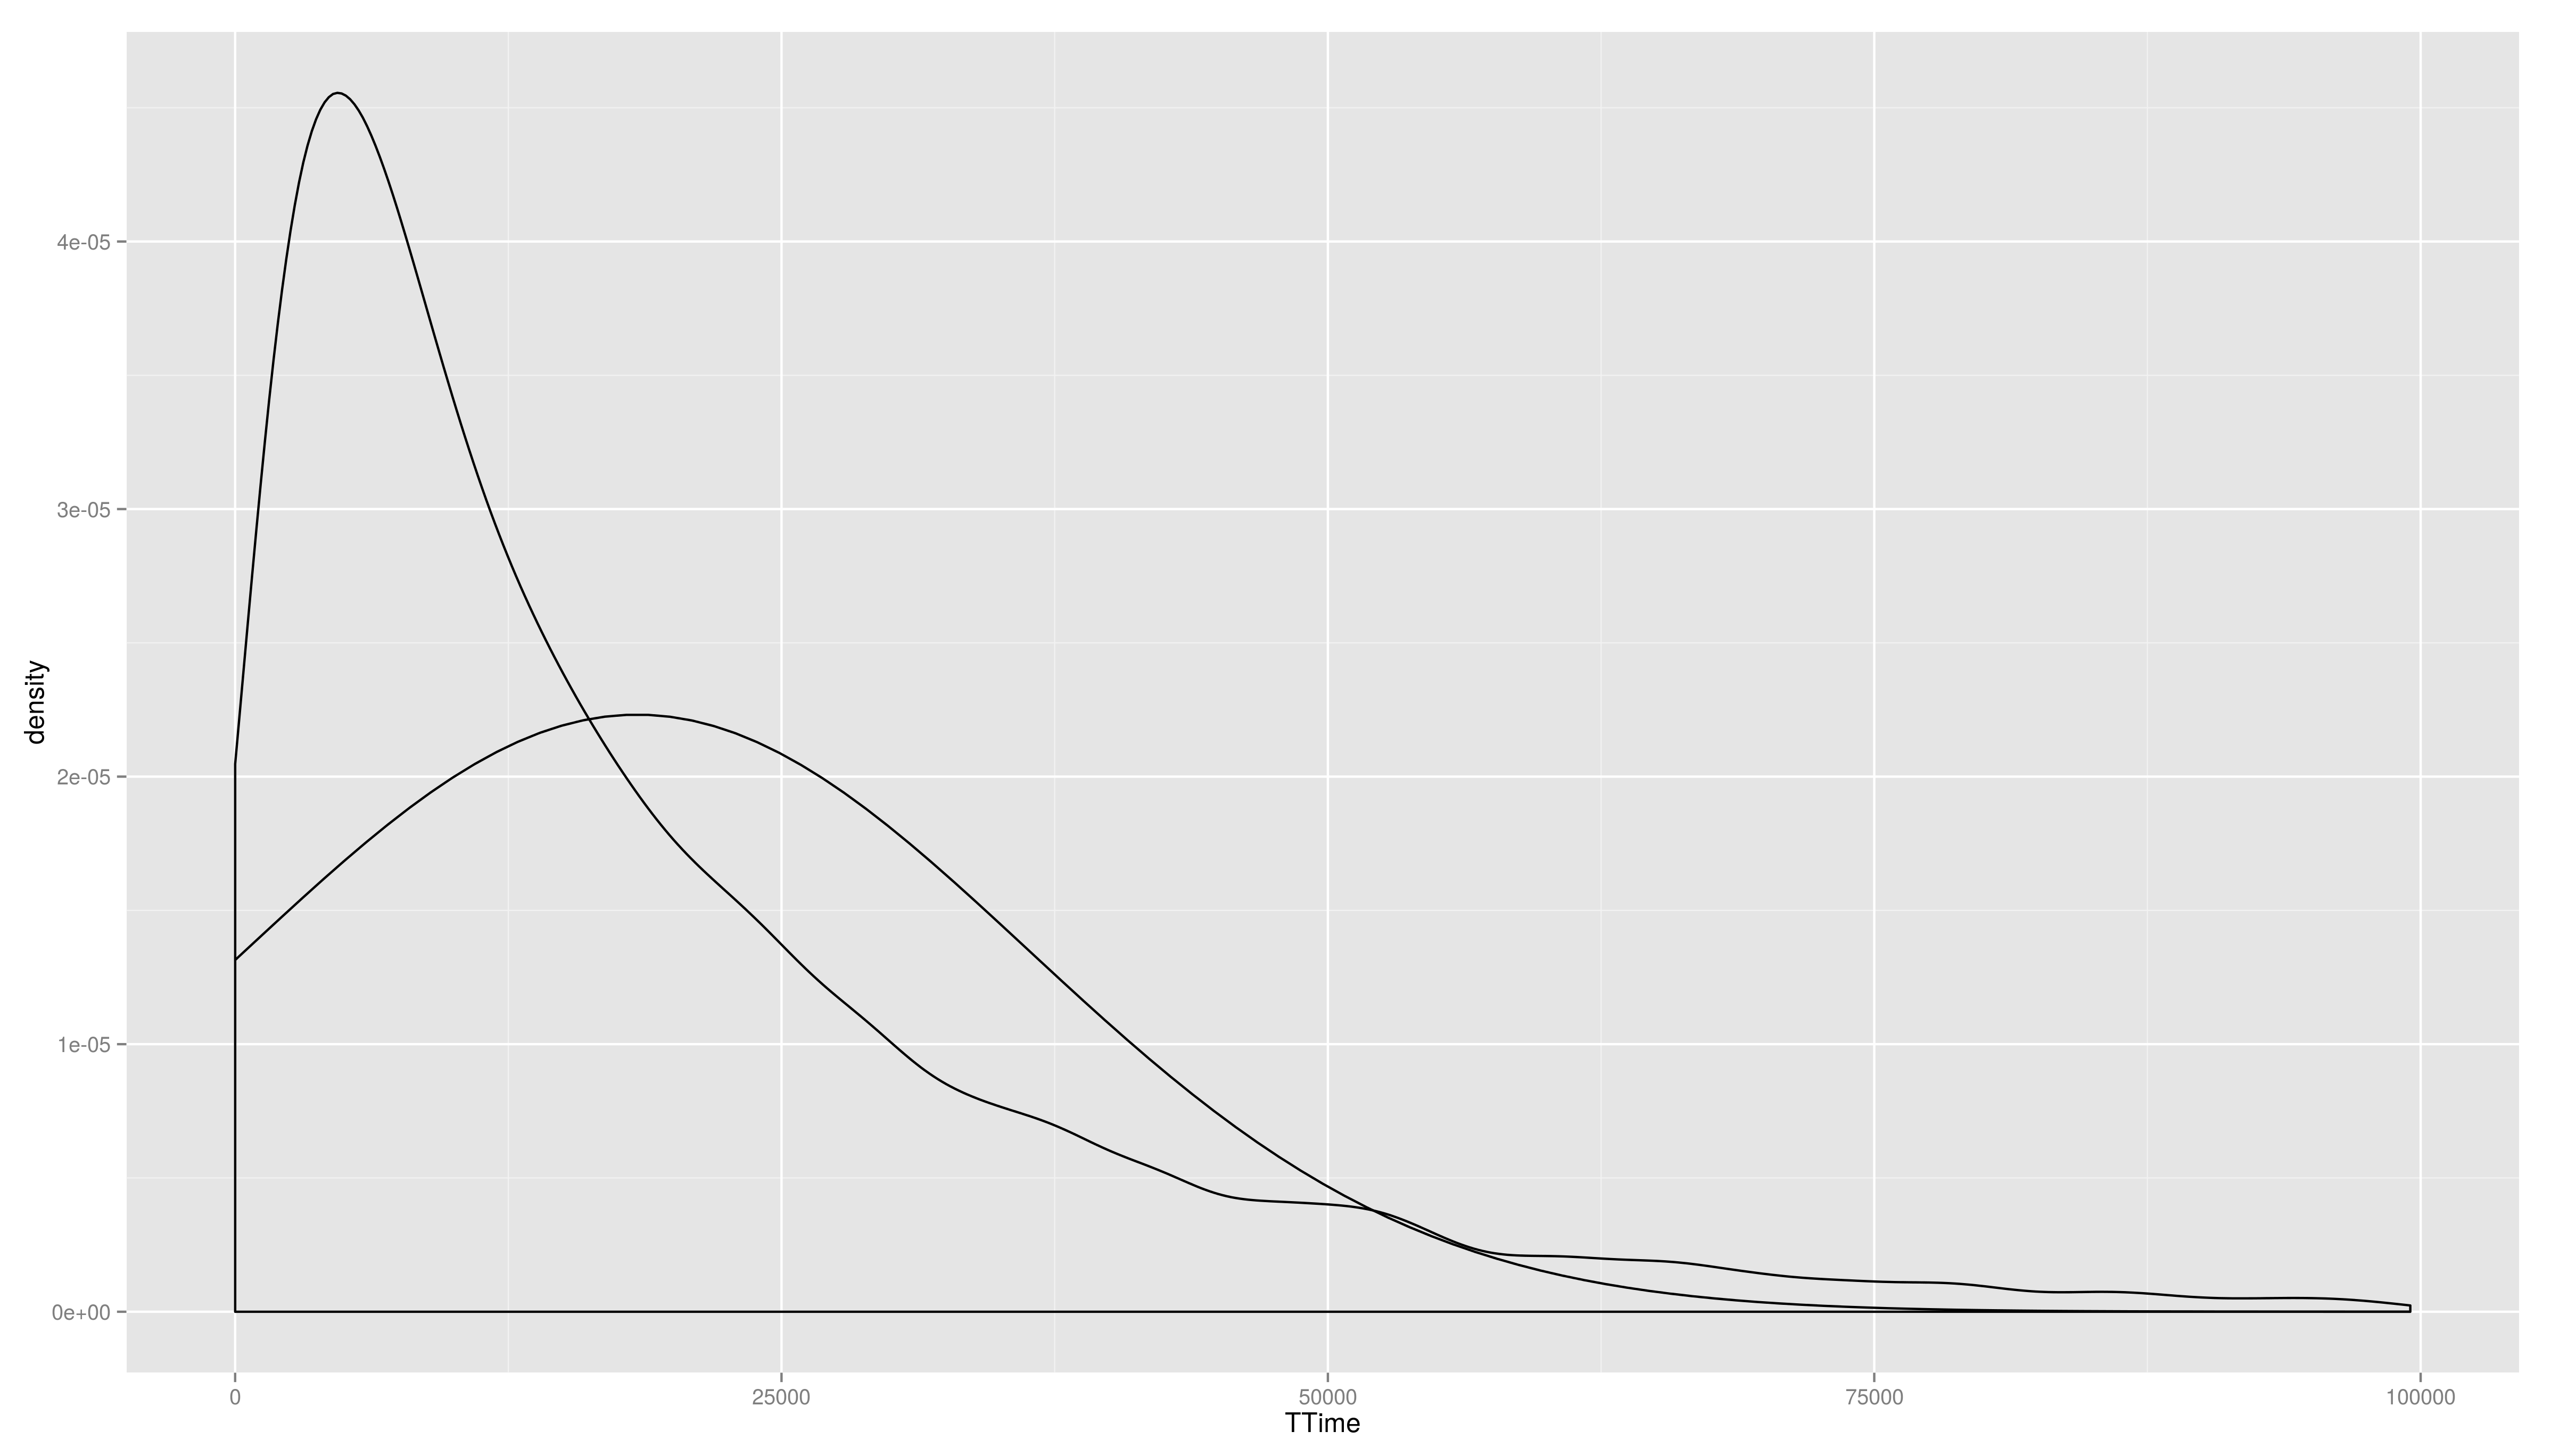
\includegraphics[width=10cm]{statdens.png}
\end{center}
\end{frame}


\begin{frame}[allowframebreaks,fragile]\frametitle{\texttt{stat\_summary()}}
  \begin{itemize}
  \item summarize y values at every unique x value
  \item default geometry: \texttt{pointrange}
  \end{itemize}
\small
\begin{verbatim}
> ggplot(data,aes(x=EC1,y=Duration)) +
+     stat_summary(fun.data="mean_se",geom = "pointrange")
\end{verbatim}
\begin{center}
  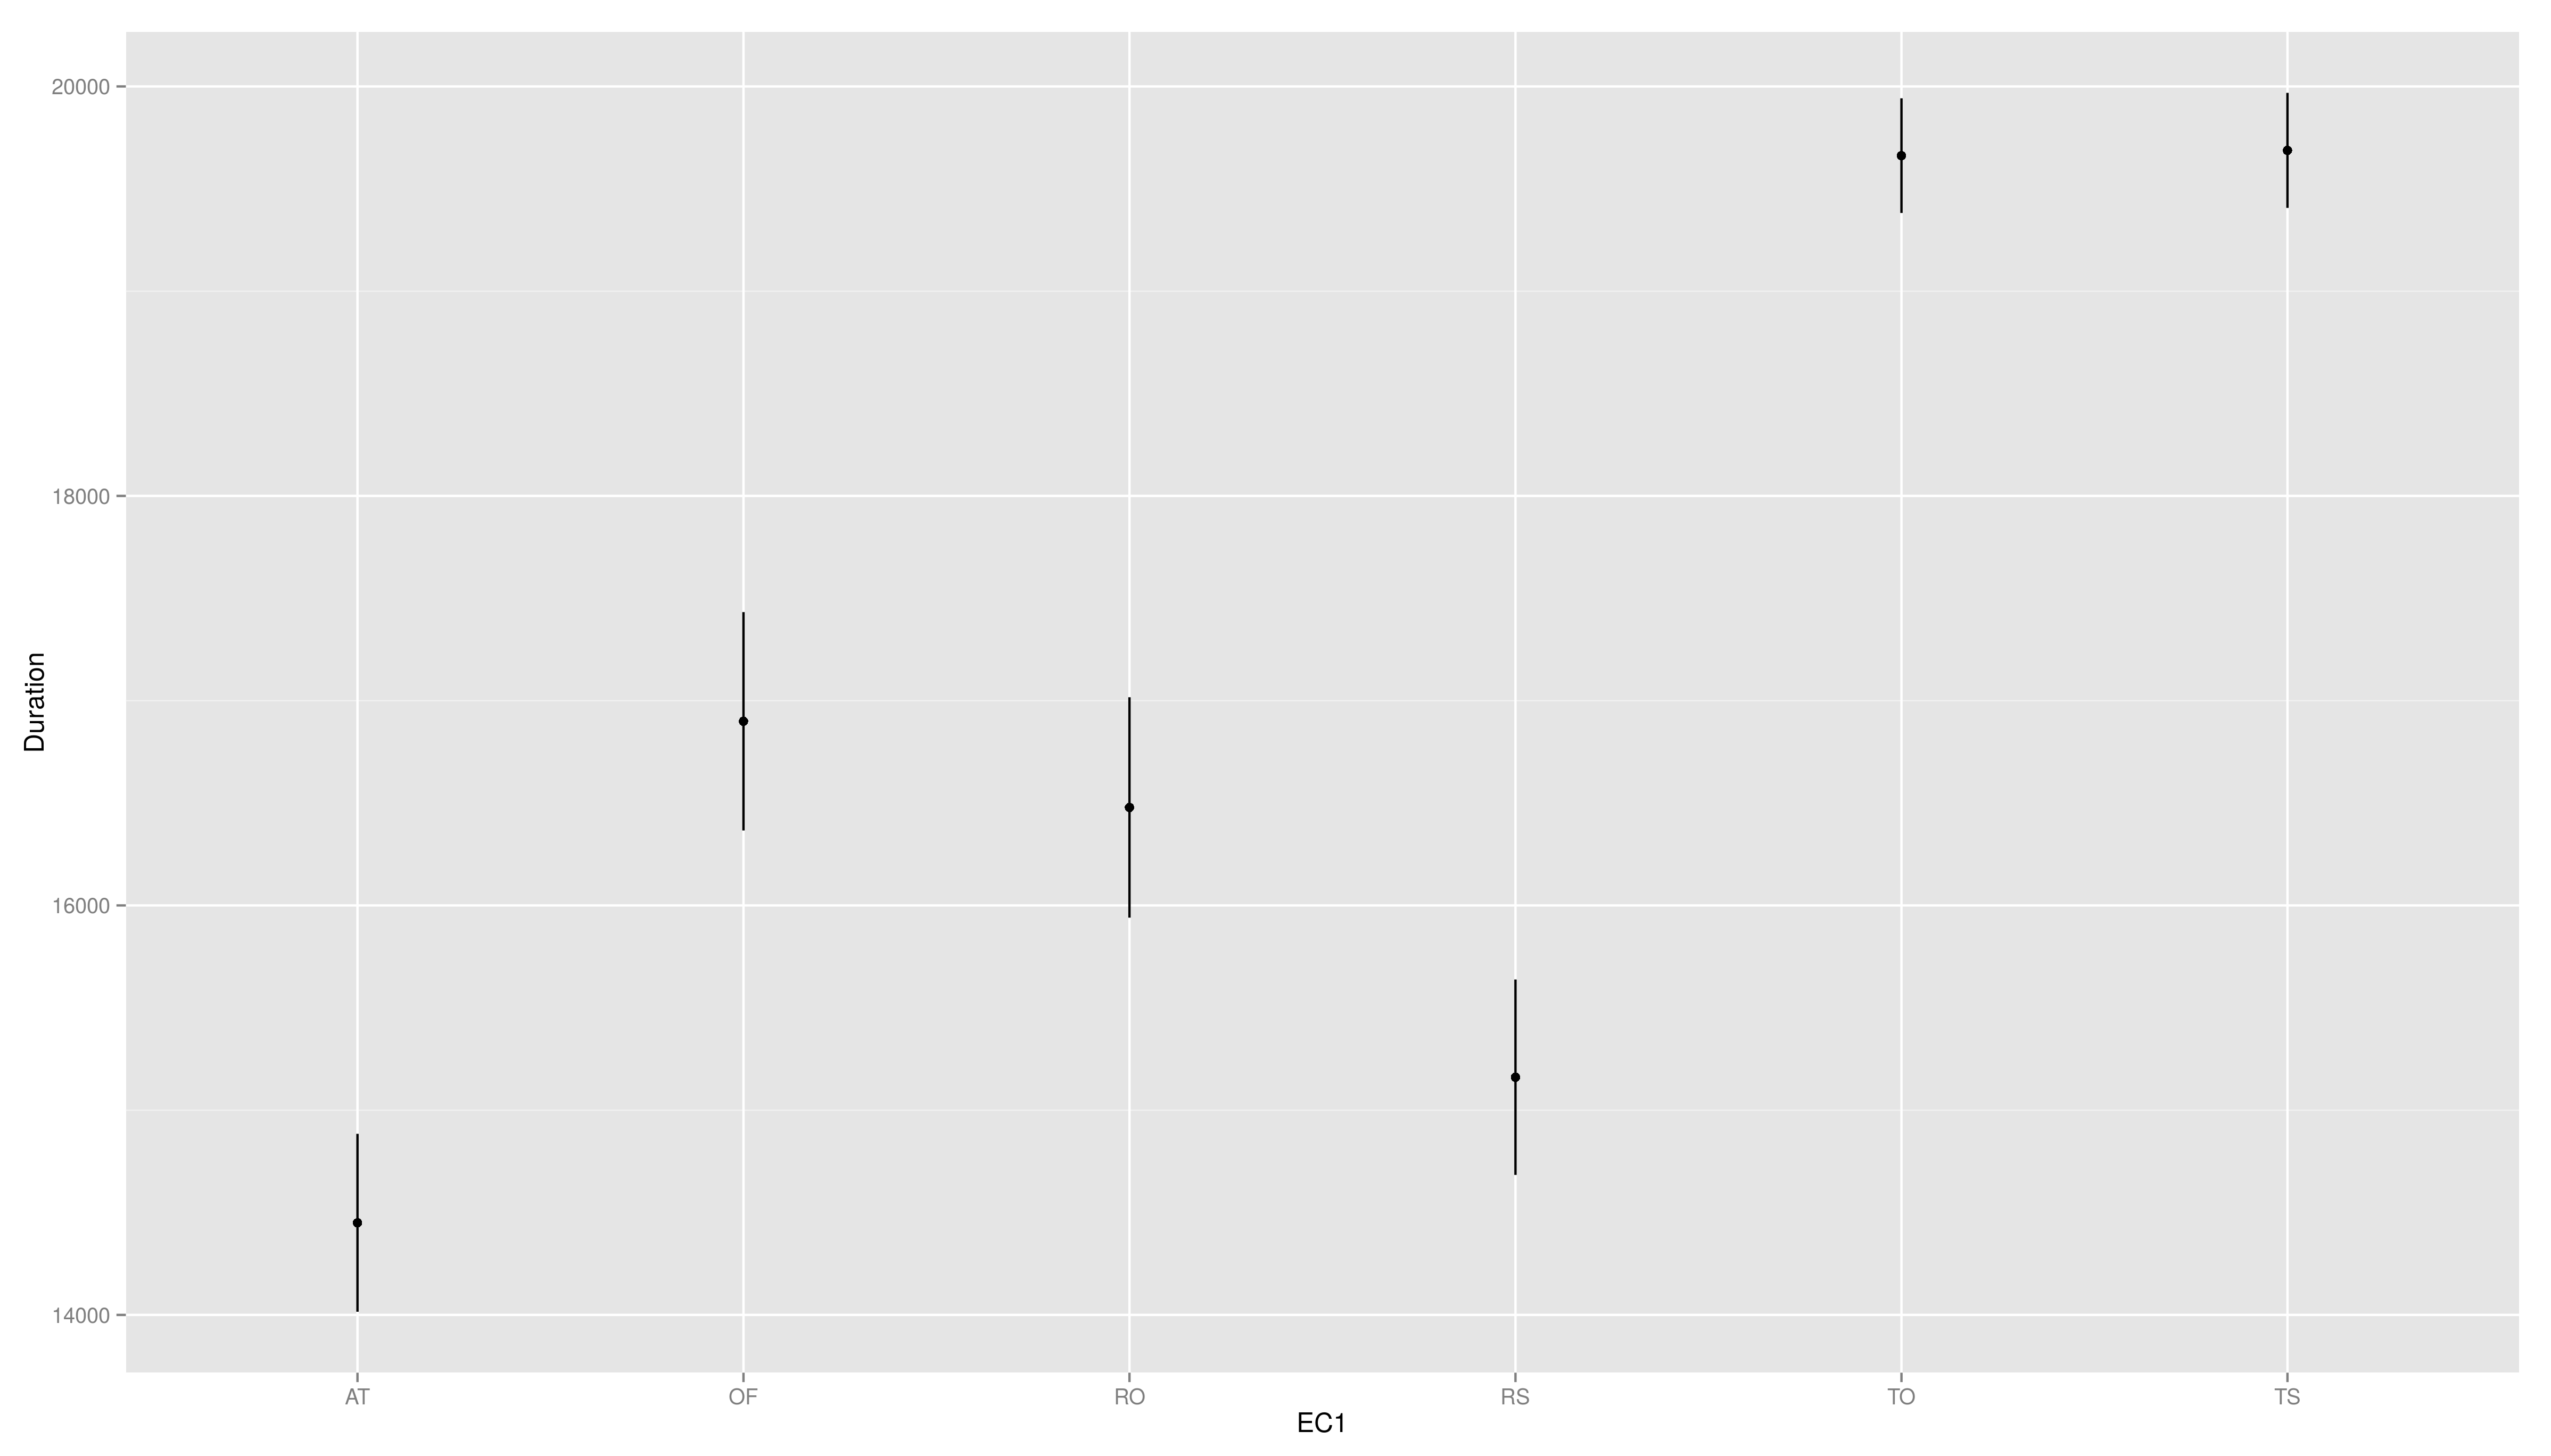
\includegraphics[width=10cm]{sum1.png}
\end{center}
\end{frame}


\begin{frame}[allowframebreaks,fragile]\frametitle{\texttt{stat\_summary()}}
  \begin{itemize}
  \item one can also create custom summary functions or stats
  \end{itemize}
\footnotesize
\begin{verbatim}
trimed.mean <- function(x){
+     data.frame(y=mean(x,na.rm = T,trim = 0.1))
+ }
> stat_meanlabel <- function(angle=0,vjust=0.5,hjust=0,...){
+     stat_summary(fun.y="mean",
+                  geom="text",
+                  aes(label=round(..y..)),
+                  hjust=hjust,
+                  vjust=vjust,
+                  angle=angle, ...)}
> ggplot(data,aes(x=EC1,y=Duration)) +
+     stat_summary(fun.data="mean_se",geom = "pointrange") +
+     stat_summary(fun.data="trimed.mean",geom = "point", colour="blue") +
+     stat_summary(fun.y="median",geom = "point", colour="green") +
+     stat_meanlabel(angle = 90,vjust = 0 )
\end{verbatim}
\begin{center}
  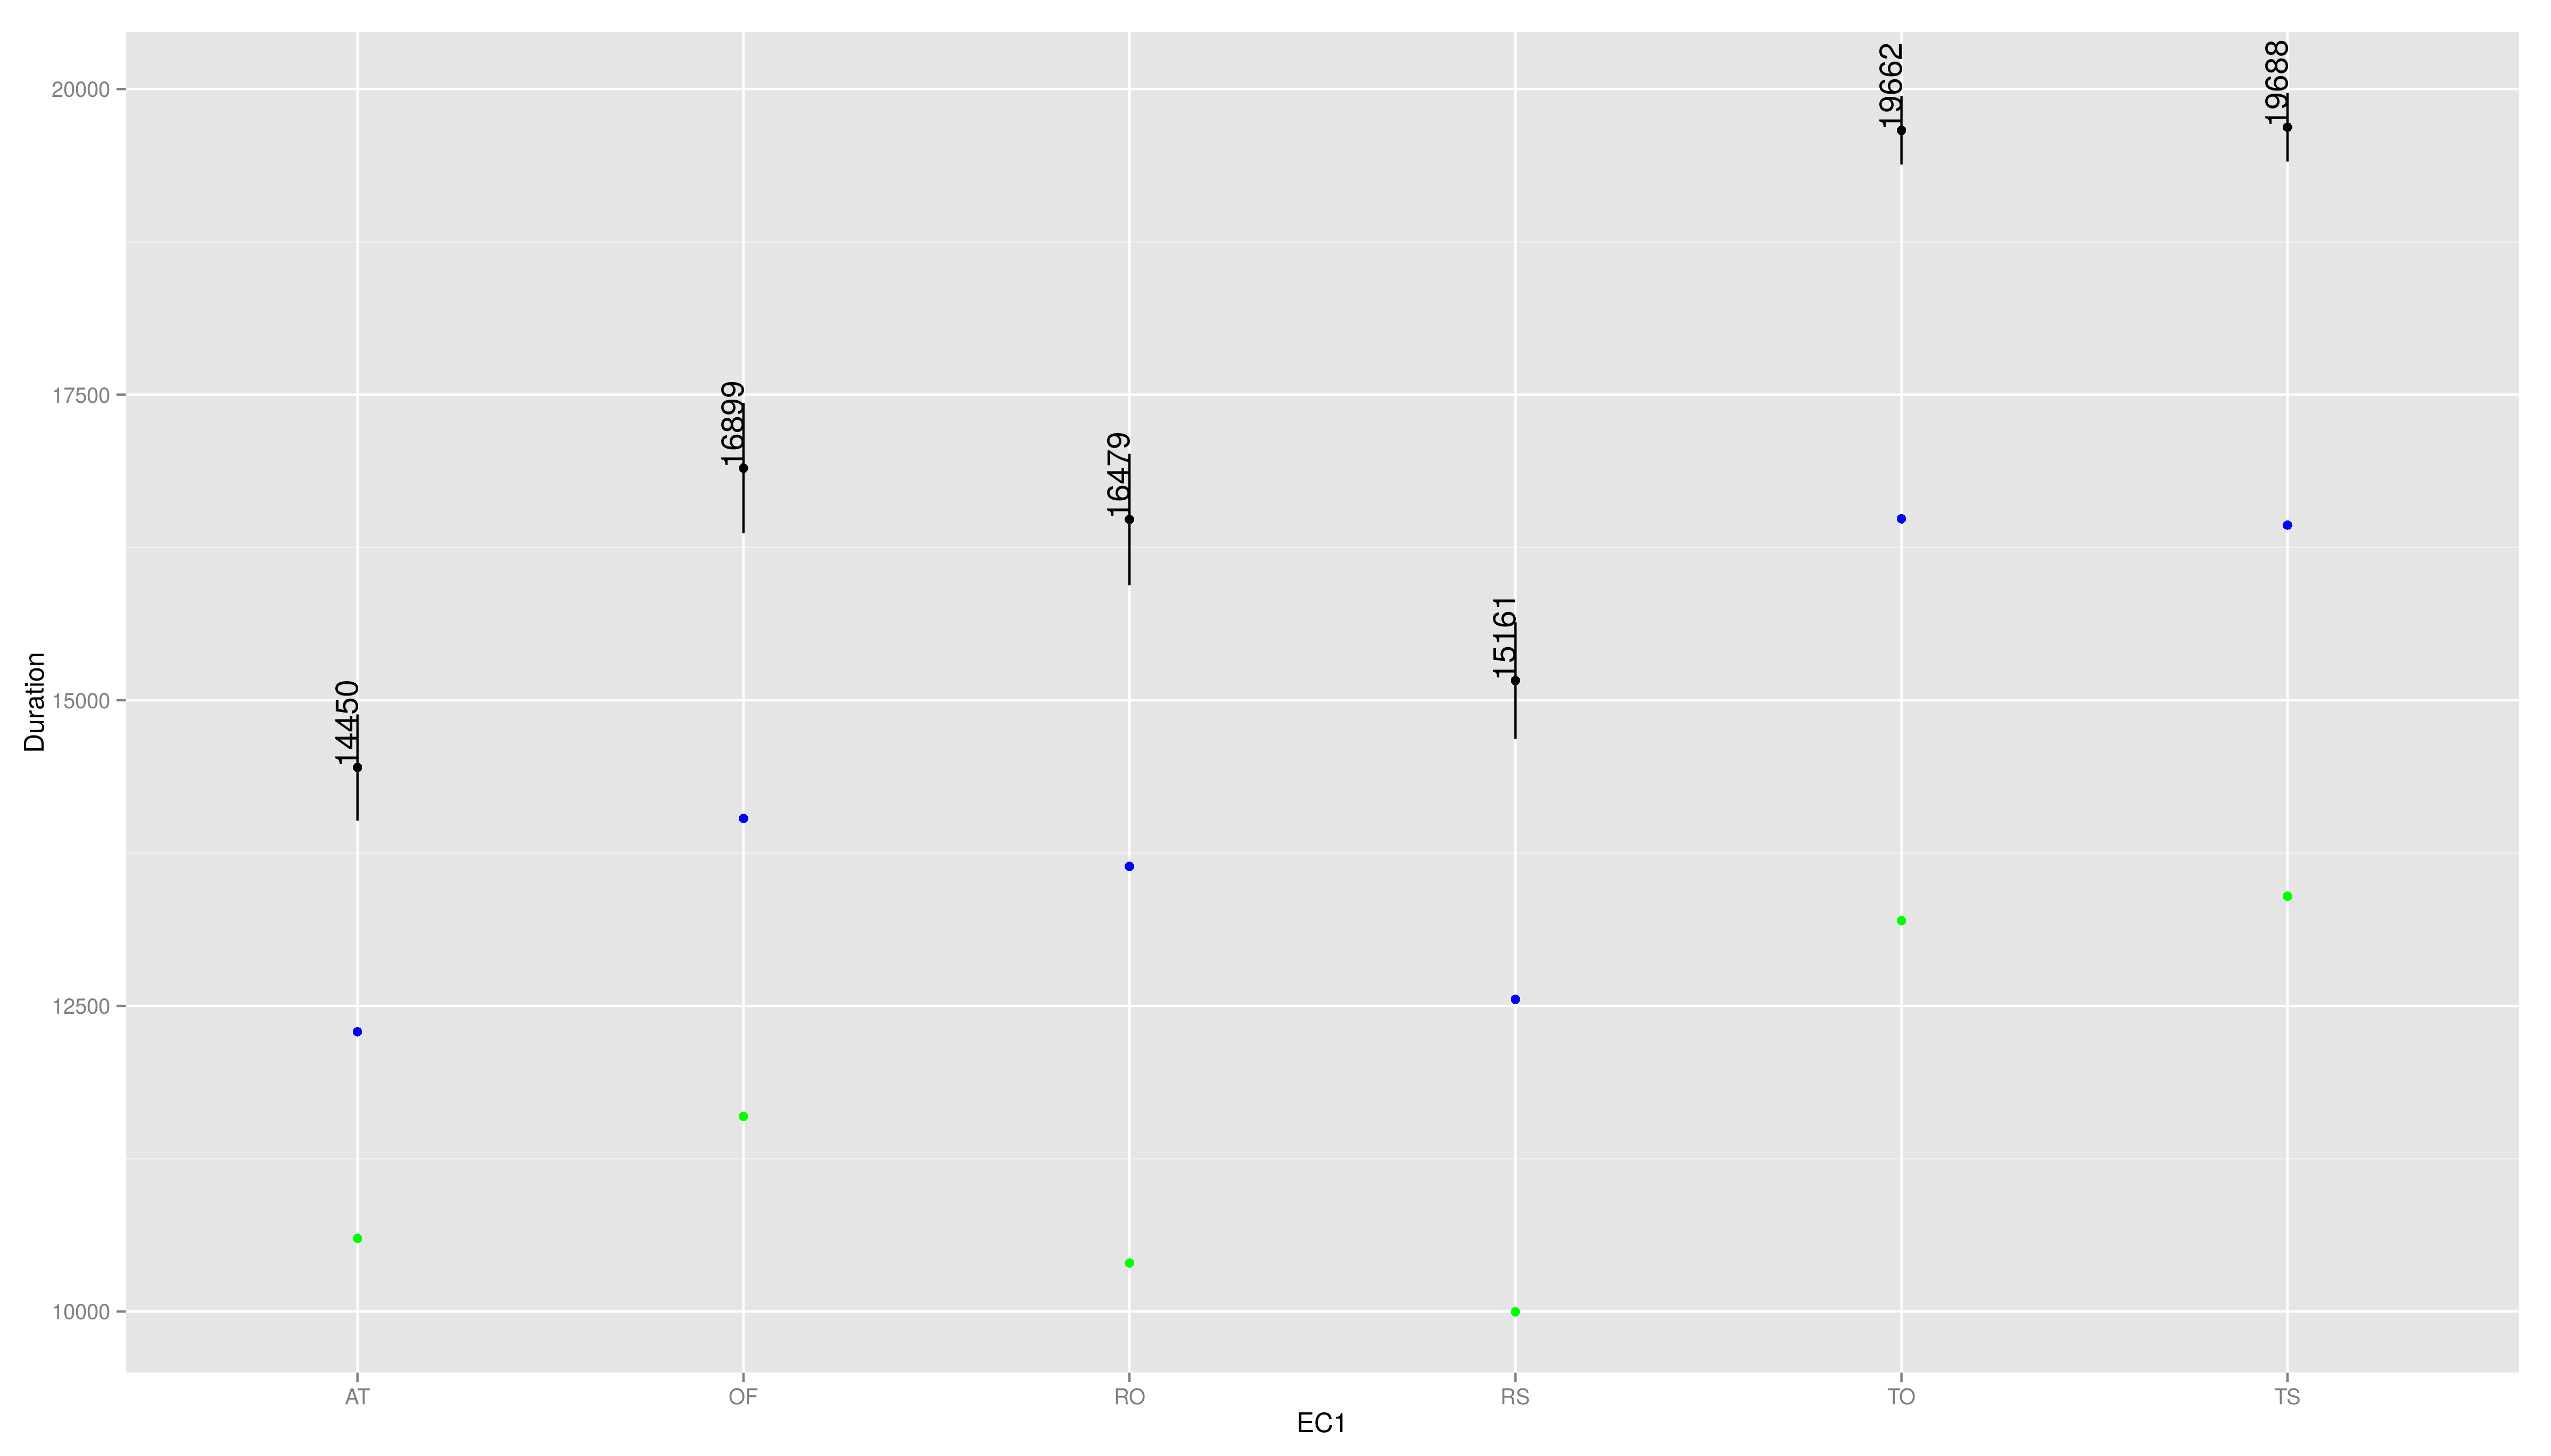
\includegraphics[width=10cm]{sum2.png}
\end{center}
\end{frame}

\subsection{Annotation}
\begin{frame}\frametitle{\texttt{annotation()}}
  \begin{itemize}
  \item creates an annotation layer (a geometry)
  \item properties of the geoms are not mapped from variables but
  \item information given as vector
  \end{itemize}
\end{frame}

